% THIS IS SIGPROC-SP.TEX - VERSION 3.1
% WORKS WITH V3.2SP OF ACM_PROC_ARTICLE-SP.CLS
% APRIL 2009
%
% Questions regarding SIGS should be sent to
% Adrienne Griscti ---> griscti@acm.org
%
% Questions/suggestions regarding the guidelines, .tex and .cls files, etc. to
% Gerald Murray ---> murray@hq.acm.org
%
% For tracking purposes - this is V3.1SP - APRIL 2009
%
% Copied from https://github.com/heathermiller/papers-documents/tree/master/rem2013

\documentclass{support/acm_proc_article-sp}
\usepackage{listings}
\usepackage{url}
\usepackage{support/bcprules}
\usepackage{support/prooftree}
\usepackage{support/math}
\usepackage{multicol}
\usepackage{caption}
\usepackage{subcaption}
\usepackage[normalem]{ulem}
\usepackage{color}
\usepackage{graphicx}
\usepackage{hyperref}

\renewcommand{\thesubsection}{\thesection.\alph{subsection}}

\definecolor{blue}{rgb}{0,0,0.5}
\definecolor{red}{rgb}{0.6,0,0}
\definecolor{green}{rgb}{0,0.5,0}
\definecolor{grey}{rgb}{0.2,0.2,0.2}

\lstdefinelanguage{Python}{
keywords={typeof, null, catch, switch, in, int, str, float, self, from, import},
keywordstyle=\color{blue}\bfseries,
ndkeywords={boolean, throw, import},
ndkeywords={return, class, if ,elif, endif, while, do, else, True, False , catch, def},
ndkeywordstyle=\color{blue}\bfseries,
identifierstyle=\color{grey},
sensitive=false,
comment=[l]{\#},
morecomment=[s]{/*}{*/},
commentstyle=\color{green}\ttfamily,
stringstyle=\color{green}\ttfamily,
}

\lstset{language=Python}

\clubpenalty = 10000
\widowpenalty = 10000
\displaywidowpenalty = 10000

% Remove copyright space
\makeatletter
\def\@copyrightspace{\relax}
\makeatother

% comments and notes
\newcommand{\comment}[1]{}
\newcommand{\note}[1]{{\bf $\clubsuit$ #1 $\spadesuit$}}
\newcommand{\ifreport}[1]{#1}
%\newcommand{\ifreport}[1]{}

\newcommand{\todo}{{\bf \colorbox{red}{\color{white}TODO:}}}
\newcommand{\ie}{{\em i.e.,~}}
\newcommand{\eg}{{\em e.g.,~}}
\newcommand{\term}[1]{\mbox{\texttt{#1}}}
\newcommand{\itl}[1]{\mbox{\textit{#1}}}

% commas and semicolons
\newcommand{\comma}{,\,}
\newcommand{\commadots}{\comma \ldots \comma}
\newcommand{\semi}{;\mbox{;};}
\newcommand{\semidots}{\semi \ldots \semi}

% spacing
\newcommand{\gap}{\quad\quad}
\newcommand{\biggap}{\quad\quad\quad}
\newcommand{\nextline}{\\ \\}
\newcommand{\htabwidth}{0.5cm}
\newcommand{\tabwidth}{1cm}
\newcommand{\htab}{\hspace{\htabwidth}}
\newcommand{\tab}{\hspace{\tabwidth}}
\newcommand{\linesep}{\ \hrulefill \ \smallskip}

\newcommand{\sectionline}{%
\nointerlineskip \vspace{\baselineskip}%
\hspace{\fill}\rule{0.5\linewidth}{.7pt}\hspace{\fill}%
\par\nointerlineskip \vspace{\baselineskip}
}

% figures
\newcommand{\figurebox}[1]
{\fbox{\begin{minipage}{\textwidth}
           #1 \medskip
\end{minipage}}}
\newcommand{\twofig}[3]
{\begin{figure*}[t]
     #3\ \hrulefill\
        \caption{\label{#1}#2}
\end{figure*}}
\newcommand{\boxfig}[3]
{\begin{figure*}
     \figurebox{#3\caption{\label{#1}#2}}
\end{figure*}}
\newcommand{\figref}[1]
{Figure~\ref{#1}}

% arrays
\newcommand{\ba}{\begin{array}}
\newcommand{\ea}{\end{array}}
\newcommand{\bda}{\[\ba}
\newcommand{\eda}{\ea\]}
\newcommand{\ei}{\end{array}}
\newcommand{\bcases}{\left\{\begin{array}{ll}}
\newcommand{\ecases}{\end{array}\right.}

\pagenumbering{arabic}
\begin{document}

    \title{Data Mining and Matrices (FSS18) \\ Assignment 4: Spectral Clustering}

    \numberofauthors{1}
    \author{
    \alignauthor
    Steffen Schmitz\\
    \affaddr{University of Mannheim}\\
    \affaddr{stefschm@mail.uni-mannheim.de}
    }

    \maketitle

    %%%%%%%%%%%%%%%%%%%%%%%%%%%%%%%%%%%%%%%%%%%%%%%%%%%%
    %%
    %% 1) Cuts
    %%
    %%%%%%%%%%%%%%%%%%%%%%%%%%%%%%%%%%%%%%%%%%%%%%%%%%%%

    \section{Cuts}

    We start by computing the values of cut (\lstinline{cut}), ratio cut (\lstinline{rcut}) and normalized cut
    (\lstinline{ncut}) for a given clustering of the $m = 500$ digits into $k = 10$ clusters.

    % Skip a and b, because they are only about implementation
    \stepcounter{subsection}
    \stepcounter{subsection}

    %%%%%%%%%%%%%%%%%%%%%%%%%%%%%%%%%%%%%%%%%%%%%%%%%%%%
    %%
    %% 1.c) Magnitude of different cuts
    %%
    %%%%%%%%%%%%%%%%%%%%%%%%%%%%%%%%%%%%%%%%%%%%%%%%%%%%

    \subsection{Magnitude of different cuts}

    \textbf{Task.} Run your \lstinline{cut} function on the \lstinline{cluster.test} clustering provided to you.
    Observe that \lstinline{cut} $\gg$ \lstinline{rcut} $\gg$ \lstinline{ncut}.
    Why is this the case?
    Is this always true?

    Considering a non-overlapping, complete clustering $C = \{C_1,\ldots, C_K\}$ of the vertices in $V$.
    Define
    \begin{equation*}
        \mbox{cut}(C) = \frac{1}{2} \sum_{k=1}^K W(C_k, V \backslash C_k) = \sum_{k=1}^K \frac{W(C_k, V \backslash C_k)}{2}
    \end{equation*}
    \begin{equation*}
        \mbox{rcut}(C) = \sum_{k=1}^K \frac{W(C_k, V \backslash C_k)}{|C_k|}
    \end{equation*}
    \begin{equation*}
        \mbox{ncut}(C) = \sum_{k=1}^K \frac{W(C_k, V \backslash C_k)}{\mbox{vol}(C_k)}.
    \end{equation*} \\
    Now, we can argue that
    \begin{equation}
        2 \ll |C_k| \ll \mbox{vol}(C_k)
        \label{eq:1c-regularization}
    \end{equation}
    should hold for almost all values $C_k \in C$.
    In our example all $|C_k|$ have a magnitude of $10^1$ and all $\mbox{vol}(C_k)$ have a magnitude of
    $10^4$, which means that the assumption in Equation~\ref{eq:1c-regularization} holds.

    Looking at $\sum_{k=1}^K 1/|C_k|$ and $\sum_{k=1}^K 1/\mbox{vol}(C_k)$ we see that they
    take their minimum, if all $|C_k|$ or all $\mbox{vol}(C_k)$ coincide, respectively~\cite[cf.p.9]{Luxburg2007}.
    On the other hand, this means that the sums are large, if the clusters are skewed.
    Then, the assumption in Equation (\ref{eq:1c-regularization}) is violated and the cut function takes a high
    value for all three variants.

    In our example, the different clusters have approximately equal size and this is also represented in the resulting
    cut values.

    %%%%%%%%%%%%%%%%%%%%%%%%%%%%%%%%%%%%%%%%%%%%%%%%%%%%
    %%
    %% 2) Similarity Graphs
    %%
    %%%%%%%%%%%%%%%%%%%%%%%%%%%%%%%%%%%%%%%%%%%%%%%%%%%%

    \section{Similarity Graphs}

    To construct a similarity graph, we make use of the Gaussian kernel (and vary parameter $\sigma$) as well as
    the various neighborhood graphs we discussed in the lecture.

    %%%%%%%%%%%%%%%%%%%%%%%%%%%%%%%%%%%%%%%%%%%%%%%%%%%%
    %%
    %% 2.a) Varying Sigma
    %%
    %%%%%%%%%%%%%%%%%%%%%%%%%%%%%%%%%%%%%%%%%%%%%%%%%%%%

    \subsection{Varying Sigma}
    \label{subsec:varying-sigma}

    \textbf{Task.} Compute the full similarity graph using $\sigma = 50$.
    Study the distribution of the resulting similarities.
    Is $\sigma = 50$ a good choice?
    Try to find a good setting for $\sigma$ by trying both smaller and larger values.
    Discuss!

    In our notebook we try the following four settings: $\sigma \in \{10, 30, 50, 70\}$.
    We can directly see that a value of $\sigma = 10$ is far too small, because there is almost no similarity between
    any numbers.
    Furthermore, the histogram shows us that there are almost no values exceeding a similarity of $0.2$.

    For $\sigma = 30$ we get the matrix shown in Figure~\ref{fig:2a-s30}.
    \begin{figure}[htbp]
        \centering
        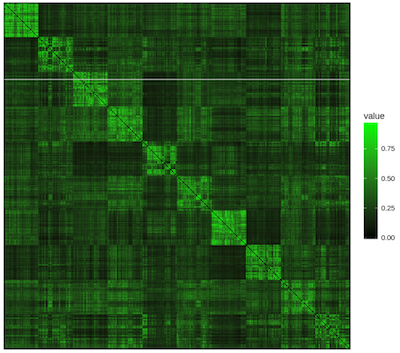
\includegraphics[width=6cm]{images/2a-s30.png}
        \caption{Matrix for $\sigma = 30$}
        \label{fig:2a-s30}
    \end{figure} \\
    The inherent structure of the matrix is clearly visible and we can directly identify the different clusters of numbers
    between which the similarity is large.
    The bell curve in the similarity histogram centers around $0.2$ and most values are in the range from $0$ to $0.5$.
    For the moment, the resulting matrix seems like a useful result.

    Next, we will look at $\sigma = 50$.
    The matrix is shown in Figure~\ref{fig:2a-s50} and the corresponding histogram in Figure~\ref{fig:2a-s50-h}.
    \begin{figure}[htbp]
        \centering
        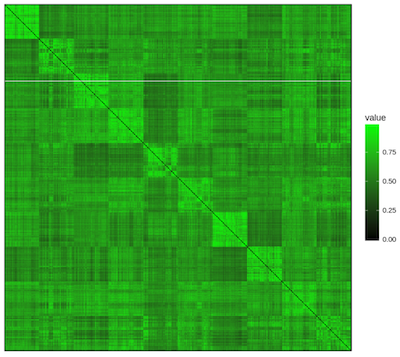
\includegraphics[width=6cm]{images/2a-s50.png}
        \caption{Matrix for $\sigma = 50$}
        \label{fig:2a-s50}
    \end{figure} \\
    We can still distinguish the different clusters in the matrix, but all other regions are also brightly green.
    The histogram centers around $0.6$, which tells us that the expected similarity between two vertices is rather high.
    \begin{figure}[htbp]
        \centering
        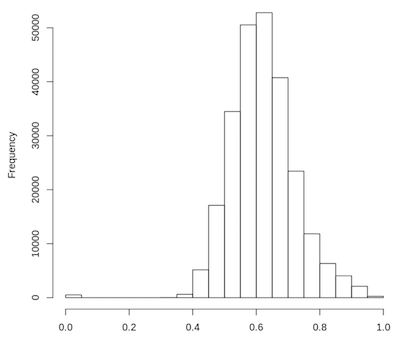
\includegraphics[width=6cm]{images/2a-s50-h.png}
        \caption{Histogram for $\sigma = 50$}
        \label{fig:2a-s50-h}
    \end{figure} \\
    Compared to the resulting matrix for $\sigma = 30$, $\sigma = 50$ does not lead to an improvement.
    Thus, the calculated similarity between two randomly selected vertices is likely to be high, even if they are dissimilar.

    Increasing the value for $\sigma$ further, makes the result even worse as we can infer from Figure~\ref{fig:2a-s70}.
    \begin{figure}[htbp]
        \centering
        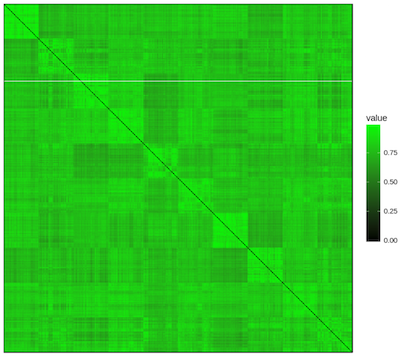
\includegraphics[width=6cm]{images/2a-s70.png}
        \caption{Histogram for $\sigma = 70$}
        \label{fig:2a-s70}
    \end{figure} \\

    Overall, the best result in our opinion provides the similarity matrix for $\sigma = 30$, as it clearly shows the clusters
    per number without assigning a high similarity to points that belong to different clusters.

    %%%%%%%%%%%%%%%%%%%%%%%%%%%%%%%%%%%%%%%%%%%%%%%%%%%%
    %%
    %% 2.b) Neighborhood Models
    %%
    %%%%%%%%%%%%%%%%%%%%%%%%%%%%%%%%%%%%%%%%%%%%%%%%%%%%

    \subsection{Neighborhood Models}
    \label{subsec:neighborhood-models}

    \textbf{Task.} For $\sigma = 50$, find the smallest $\epsilon$ such that the $\epsilon$-neighborhood graph is
    connected.
    Note that you can use the magnitudes of the smallest eigenvalues of the Laplacian to judge whether or not the graph
    is connected.
    Now find the smallest $k$ such that the symmetric kNN graph is connected, and the smallest $k$ such that the mutual
    kNN graph is connected.
    Plot the resulting similarity matrices.
    Are they different?
    If so, why?
    Discuss!

    "A graph [\ldots] is connected [\ldots] [if] there is a path from any point to any other point in
    the graph"~\cite{Weissstein2018}.
    If we arrange all the eigenvalues of the Laplacian in non-increasing order, i.e.\@:
    \begin{equation*}
        \lambda_1 \geq \lambda_2 \geq \ldots \geq \lambda_{n-1} \geq \lambda_n = 0
    \end{equation*}
    we can apply the matrix-tree theorem and say that the graph is connected, iff
    $\lambda_{n-1} > 0$~\cite[cf.p.3]{Zhang2011}.

    In our notebook we pick some parameters for $\epsilon$ and $k$ and increase or decrease them until we find the lowest
    value for which $\lambda_{n-1}$ is greater than zero.

    The resulting similarity matrices are shown in
    Figure~\ref{fig:2b-e-neighbors},~\ref{fig:2b-symmetric-knn} and~\ref{fig:2b-mutual-knn}.
    \begin{figure}[htbp]
        \centering
        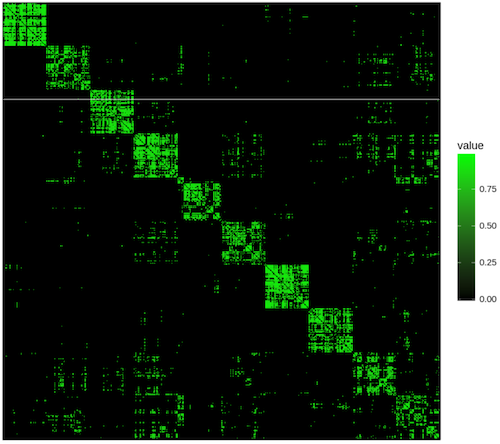
\includegraphics[width=6cm]{images/2b-e-neighbors.png}
        \caption{$\epsilon$-neighborhood}
        \label{fig:2b-e-neighbors}
    \end{figure}
    \begin{figure}[htbp]
        \centering
        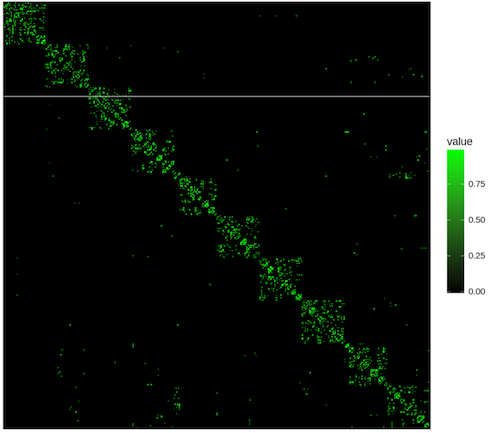
\includegraphics[width=6cm]{images/2b-symmetric-knn.png}
        \caption{Symmetric kNN}
        \label{fig:2b-symmetric-knn}
    \end{figure}
    \begin{figure}[htbp]
        \centering
        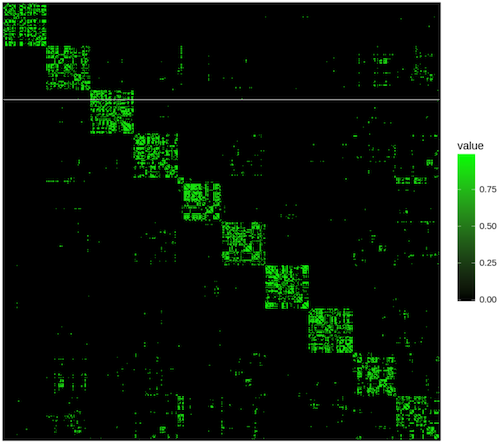
\includegraphics[width=6cm]{images/2b-mutual-knn.png}
        \caption{Mutual kNN}
        \label{fig:2b-mutual-knn}
    \end{figure}
    The $\epsilon$-neighborhood and mutual kNN graphs look similar and have approximately the same shapes and
    densities.
    Their plot contains ten obvious clusters, each representing one number, and some noise in the top right and
    bottom left.

    On the other hand, the symmetric kNN graph has very little green regions, except for the clusters we
    already recognized in the other two plots.

    Our assumption is that the symmetric kNN graph is more likely to jump to other clusters and, therefore,
    connects the whole graph more quickly, while the mutual kNN and $\epsilon$-neighborhood graph completely connect
    a cluster, before jumping to another one.
    This explains why the similarity matrices for mutual kNN and $\epsilon$-neighborhood have a higher density
    around the actual clusters and why they show more noise.

    %%%%%%%%%%%%%%%%%%%%%%%%%%%%%%%%%%%%%%%%%%%%%%%%%%%%
    %%
    %% 2.c) Parameters for Symmetric KNN
    %%
    %%%%%%%%%%%%%%%%%%%%%%%%%%%%%%%%%%%%%%%%%%%%%%%%%%%%

    \subsection{Parameters for Symmetric KNN}
    \label{subsec:parameters}

    \textbf{Task.} For the symmetric $k$-nearest neighbor graph, manually determine values for $\sigma$ and $k$ that
    appear suitable to you.

    In Section~\ref{subsec:varying-sigma} we found that $\sigma = 30$ is a good choice and a general recommendation for
    a first pick of $k$ is $\log(n)$, which is $2.69$ or roughly $3$ in our case.
    Using this as our first pick we obtain the similarity matrix in Figure~\ref{fig:2c-s30-k3}.
    \begin{figure}[htbp]
        \centering
        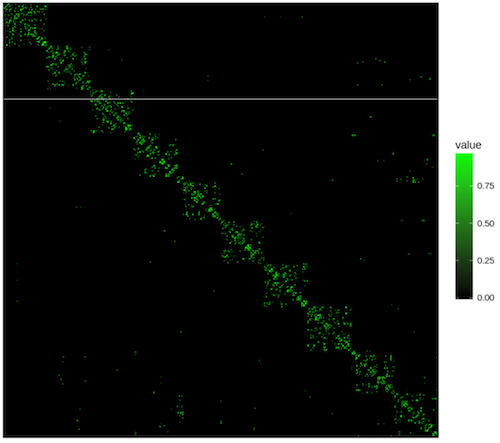
\includegraphics[width=6cm]{images/2c-s30-k3.png}
        \caption{Symmetric kNN with s=30 and k=3}
        \label{fig:2c-s30-k3}
    \end{figure}
    From the eigenvalues of the Laplacian we can directly see that the graph is not connected,
    because $\lambda_{n-1}$ is zero.
    The resulting matrix looks even more sparse than the parameter configuration that we used
    for Figure~\ref{fig:2b-symmetric-knn}.

    "In general, if the similarity graph contains more connected components than the number of clusters we ask the
    algorithm to detect, then spectral clustering will trivially return connected components as clusters.
    Unless one is perfectly sure that those connected components are the correct clusters, one should make sure
    that the similarity graph is connected"~\cite[p.21]{Luxburg2007}.
    Although we are convinced that each connected component belongs into a cluster, we want to be absolutely sure.
    Following the insights from von Luxburg, we, therefore, should aim for a connected graph that is more
    densely populated than the previously computed ones.

    We will now try to increase the number of clusters until the graph is fully connected and
    find that $k = 4$ leads to a connected graph and that the graph looks even more similar to the one in
    Figure~\ref{fig:2b-symmetric-knn}.
    Increasing $\sigma$ to 80 also results in a similar matrix and the graph is still connected.

    Hence, we will continue to increase $k$, while keeping $\sigma = 30$, because an increasement of $\sigma$ had no
    visible effect.
    With increasing $k$ the resulting matrix approximates the results that we got for $\epsilon$-neighborhood and
    mutual kNN in Section~\ref{subsec:neighborhood-models}.
    The clusters become more dense, but the noise also increases.
    In our opinion, $k = 25$ and $\sigma = 30$ is a good parameter combination that captures the clusters well, while
    keeping the noise low.
    The result is shown in Figure~\ref{fig:2c-s30-k25}.
    \begin{figure}[htbp]
        \centering
        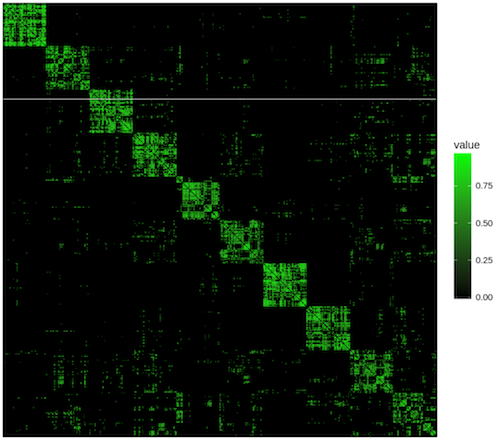
\includegraphics[width=6cm]{images/2c-s30-k25.png}
        \caption{Symmetric kNN with s=30 and k=25}
        \label{fig:2c-s30-k25}
    \end{figure}

    %%%%%%%%%%%%%%%%%%%%%%%%%%%%%%%%%%%%%%%%%%%%%%%%%%%%
    %%
    %% 2.d) Influence of sigma
    %%
    %%%%%%%%%%%%%%%%%%%%%%%%%%%%%%%%%%%%%%%%%%%%%%%%%%%%

    \subsection{Influence of sigma}

    \textbf{Task.} Consider any dataset in Euclidean space.
    Suppose that we use the Gaussian kernel with parameter $\sigma$ to obtain similarities and subsequently construct
    a symmetric $k$-nearest neighbor graph.
    Describe what changes to expect in the so-obtained graph when we increase or decrease $\sigma$.
    Is there anything that does not change?

    The Gaussian kernel is defined as
    \begin{equation*}
        w_{ij} = \exp{\left(\frac{-\delta_{ij}^2}{2\sigma^2}\right)}
    \end{equation*}
    and the parameter $\sigma$ controls what is considered local.
    This function assigns a value of 1 if the distance is 0 and approximates 0 asymptotically for even larger values.
    We can control the steepness of the decline with $\sigma$.

    The Gaussian kernel function is approximately linear around its inflection point and flattens out at the edges.
    We assume that a change in the value of $\sigma$ mostly affects points that are very close.

    We suppose that $x_1$ and $x_2$ are part of a dataset in Eucledian space with $x_0$.
    If both are far away, both weights $w_{01}$ and $w_{02}$ will be small for any $\sigma$ and negligible, because
    they are unlikely to be neighbors.
    In the case that the distance between $x_1$ and $x_2$ is around the inflection point for any $\sigma$ the resulting
    weight will reflect the distance between them and $x_0$ almost linearly and, therefore, will not have a big influence.
    We only recognize a significant influence of $\sigma$ on the similarity, if both points are very close to $x_0$.
    In this case, they will seem far apart for small $\sigma$s and the distance is amplified due to
    the steep decline.
    Alternatively, they may appear closer together for large values of $\sigma$, because the Gaussian kernel
    is approximately flat for small distances.

    With symmetric kNN it is guaranteed that each vertex has at least $k$ neighbors.
    We assume that we have far more connections for a large $\sigma$, because nearby matrices seem even closer due to
    the flat behavior of the kernel function.
    On the other hand, we expect the number of neighbors to drop for very small $\sigma$.
    The only thing that does not change is the similarity that we expect for vertices that are far apart.
    We should always assign a small similarity value to them.

    %%%%%%%%%%%%%%%%%%%%%%%%%%%%%%%%%%%%%%%%%%%%%%%%%%%%
    %%
    %% 3) Spectral Clustering
    %%
    %%%%%%%%%%%%%%%%%%%%%%%%%%%%%%%%%%%%%%%%%%%%%%%%%%%%

    \section{Spectral Clustering}

    In this experiment, we try to cluster the digit data into 10 different clusters;
    the "optimal" clustering assigns the same digits to the same cluster, and different digits to
    different clusters.

    %%%%%%%%%%%%%%%%%%%%%%%%%%%%%%%%%%%%%%%%%%%%%%%%%%%%
    %%
    %% 3.a) k-means
    %%
    %%%%%%%%%%%%%%%%%%%%%%%%%%%%%%%%%%%%%%%%%%%%%%%%%%%%

    \subsection{k-means}
    \label{subsec:k-means}

    \textbf{Task.} First cluster the digits data using $k$-means on both the raw data and the first 10
    principal component scores.
    Visualize the result and compute the accuracy.
    Are the results good?
    Which "errors" are made?

    Running $k$-means on the raw input data with $k = 10$ clusters results in an accuracy of $82.4\%$.
    From the confusion matrix we see that many 9s are incorrectly labeled as 3s, 1s are often confused for 8s
    and k-means often predicts a 4 for a 9.
    Although the input dataset is balanced, k-means labels more than 80 images as 3 and less than 40 images
    as either 1 or 4.

    k-means works best, if all clusters are of globular shape and have a strict separation.
    Yet, the results indicate that this is not the case for the digits dataset.
    Especially the clusters for 9 and 3, 1 and 8 and 4 and 9 seem to overlap.

    We observe the same behavior for the k-means clustering on the first 10 PCA scores.
    The accuracy is down to $80\%$ and the confusion matrix is similar to the previous one.
    We conclude that the effect of overlapping clusters is only amplified by the reduction to ten dimensions.

    %%%%%%%%%%%%%%%%%%%%%%%%%%%%%%%%%%%%%%%%%%%%%%%%%%%%
    %%
    %% 3.b) First Run of Spectral Clustering
    %%
    %%%%%%%%%%%%%%%%%%%%%%%%%%%%%%%%%%%%%%%%%%%%%%%%%%%%

    \subsection{First run of Spectral Clustering}
    \label{subsec:spectral-clustering}

    \textbf{Task.} Use your parameter settings of task 2c) and run spectral clustering.
    Compare the result with the results obtained above.
    Which method worked best?
    Did your parameter settings produce good results?
    Which "errors" are made?

    Using spectral clustering we obtain an accuracy of $83.6\%$ and, therefore, see an improvement on both of the results
    we obtained in the previous subsection.
    The combinations of problematic pairs that we identified in Section~\ref{subsec:k-means} are critical, again.
    Nevertheless, the improvement shows that spectral clustering is an improvement over $k$-means on the raw
    data.

    Looking again at Figure~\ref{fig:2c-s30-k25}, we also see that most of the noise is in the 4th, 9th and 10th
    row.
    This may indicate that those regions still are very similar and that the graph is not sparse enough.
    Hence, we draw the conclusion that our selection for $k$ was too big and that we should try a smaller $k$
    for our optimization attempt that follows in Section~\ref{subsec:parameter-tuning}.

    %%%%%%%%%%%%%%%%%%%%%%%%%%%%%%%%%%%%%%%%%%%%%%%%%%%%
    %%
    %% 3.c) Eigengap Heuristic
    %%
    %%%%%%%%%%%%%%%%%%%%%%%%%%%%%%%%%%%%%%%%%%%%%%%%%%%%

    \subsection{Eigengap Heuristic}

    \textbf{Task.} In practice, we may not know the optimal number of clusters.
    Use the eigengap heuristic to estimate a good choice for the number of clusters.
    Discuss!

    For this task, we will again use the parameter combination from
    Section~\ref{subsec:parameters}, $k = 25$ and $\sigma = 30$.
    The 100 smallest eigenvalues are plotted in Figure~\ref{fig:3c-eigenvalues}.
    \begin{figure}[htbp]
        \centering
        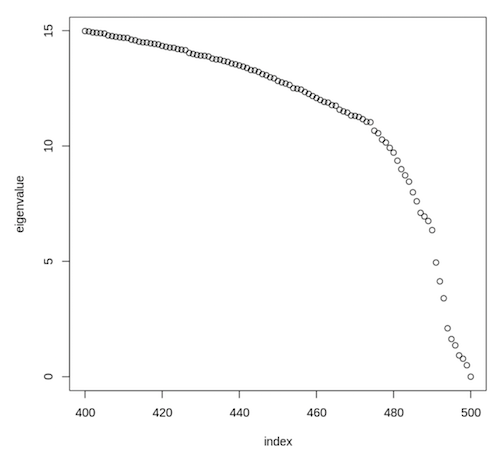
\includegraphics[width=6cm]{images/3c-eigenvalues.png}
        \caption{Last 100 eigenvalues}
        \label{fig:3c-eigenvalues}
    \end{figure}
    According to the eigengap-heuristic we should select a number of clusters $k$ such that
    $\lambda_1,\ldots,\lambda_{n-k}$ are large and $\lambda_{n - k + 1},\ldots,\lambda_n$ are small.
    In the eigenvalue chart, we see that there is a gap after the last 7 and after the last 10 eigenvalues.

    Taking the first larger gap as our guidance, we would select $k = 7$ for the clustering algorithm.
    This also fits our observation from the previous subsection that 9 and 3, 1 and 8 and 4 and 9 seem to overlap.
    Applying the eigengap heuristic, we effectively find about seven clusters with the current parameter setting.

    %%%%%%%%%%%%%%%%%%%%%%%%%%%%%%%%%%%%%%%%%%%%%%%%%%%%
    %%
    %% 3.d) Parameter Tuning
    %%
    %%%%%%%%%%%%%%%%%%%%%%%%%%%%%%%%%%%%%%%%%%%%%%%%%%%%

    \subsection{Parameter Tuning}
    \label{subsec:parameter-tuning}

    \textbf{Task.} Now "tune" the parameters of spectral clustering with 10 clusters to obtain an accuracy
    above 0.88.
    Why do you think that the so-obtained parameters work well?

    First, we will follow our intuition from Section~\ref{subsec:spectral-clustering} and decrease the
    number of $k$ that we use for our symmetric kNN graph.
    We already found that the graph is connected for $k = 4$ and while trying values around $k = 4$, we find
    that $k = 5$ yields a good result with an accuracy of $89.6\%$.
    Hence, we draw the conclusion that spectral clustering works best if the graph is very sparse,
    but connected.

    Starting from $\sigma = 30$ we first go up to 50, 100 and 200 without seeing any change in the accuracy and
    afterwards down to 5 and 10.
    For $\sigma = 5$ the accuracy is very low and an indication that $\sigma$ is too small to reflect the
    similarities accurately.
    With this parameter setting every point seems dissimilar to every other.
    On the other hand, we improve our accuracy to $91.4\%$ with $\sigma = 10$.
    We assume that this parameter setting reflects the locality in the graph in the most accurate way.
    Lower values of $\sigma$ lead to a low similarity for too many points, while a higher value of $\sigma$
    probably returns a high similarity for points, even if they belong into other, nearby clusters.

    The resulting matrix with our optimized parameters is shown in Figure~\ref{fig:3d-optimal}.
    \begin{figure}[htbp]
        \centering
        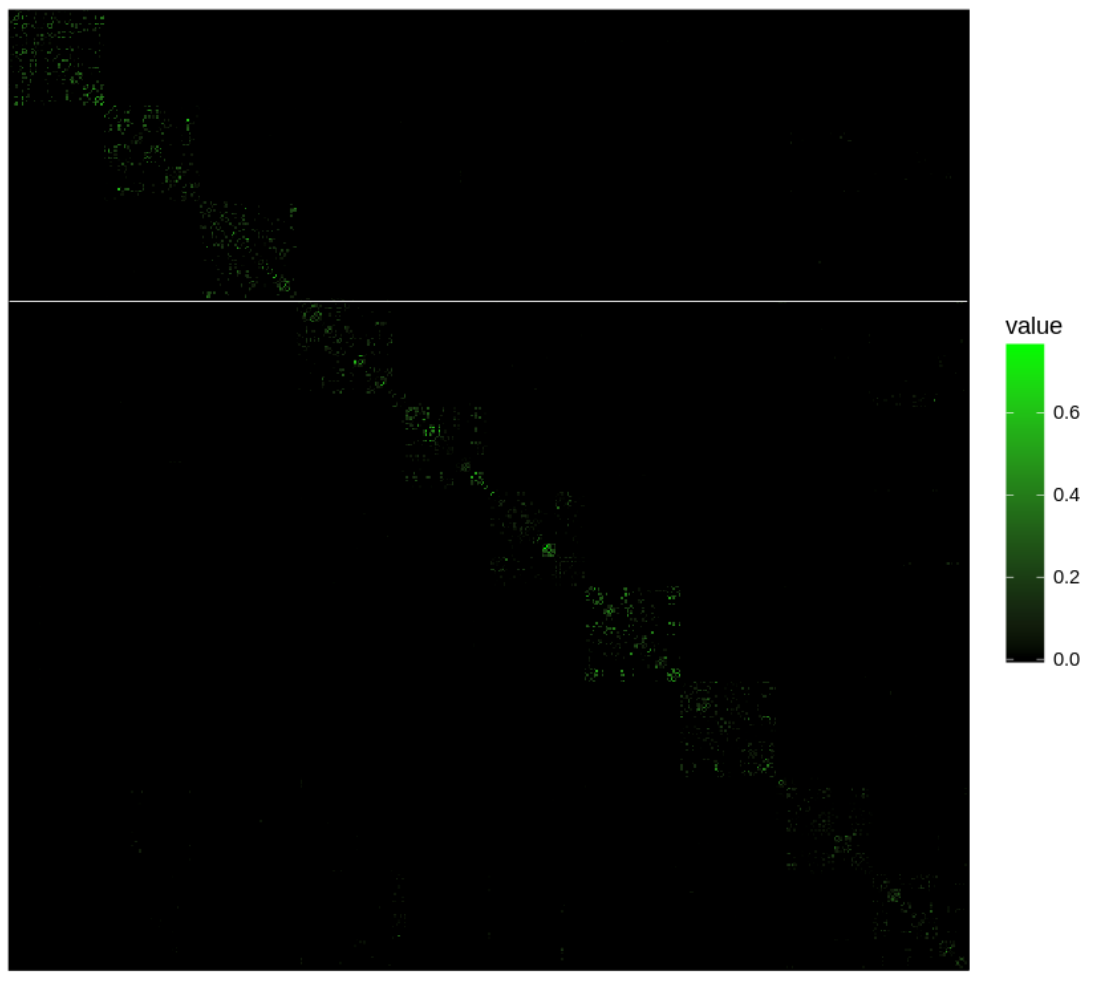
\includegraphics[width=6cm]{images/3d-optimal.png}
        \caption{Symmetric kNN with s=10 and k=5}
        \label{fig:3d-optimal}
    \end{figure}
    Surprisingly, this matrix is very sparse.
    This shows that our assumptions from Section~\ref{subsec:varying-sigma} are not correct and it is an advantage
    if the clusters are not densely connected.

    Overall, a small $k$ that connects the full graph, while maintaining sparseness, seems to be a good choice
    and $\sigma$ should be selected in such a way that it allows neighbors be close, while returning a low similarity for
    points that are further away.

    %%%%%%%%%%%%%%%%%%%%%%%%%%%%%%%%%%%%%%%%%%%%%%%%%%%%
    %%
    %% BIBLIOGRAPHY
    %%
    %%%%%%%%%%%%%%%%%%%%%%%%%%%%%%%%%%%%%%%%%%%%%%%%%%%%

    \bibliographystyle{abbrv}
    \bibliography{support/bib}

\end{document}
